% ============================================================================
% SEC02.TEX - Section 4.2: Membuat Player GameObject
% ============================================================================

\section{Membuat Player GameObject}

Setelah project siap, kita akan membuat karakter utama: pesawat luar angkasa.

\subsection{Membuat Sprite Player}

\begin{enumerate}
    \item Di panel \textbf{Hierarchy}, klik kanan > \textbf{2D Object} > \textbf{Sprites} > \textbf{Triangle}.
    \item Beri nama objek tersebut \texttt{Player}.
    \item Pastikan posisi (Position) di \textbf{Transform} adalah $(0, 0, 0)$.
    \begin{figure}[ht]
        \centering
        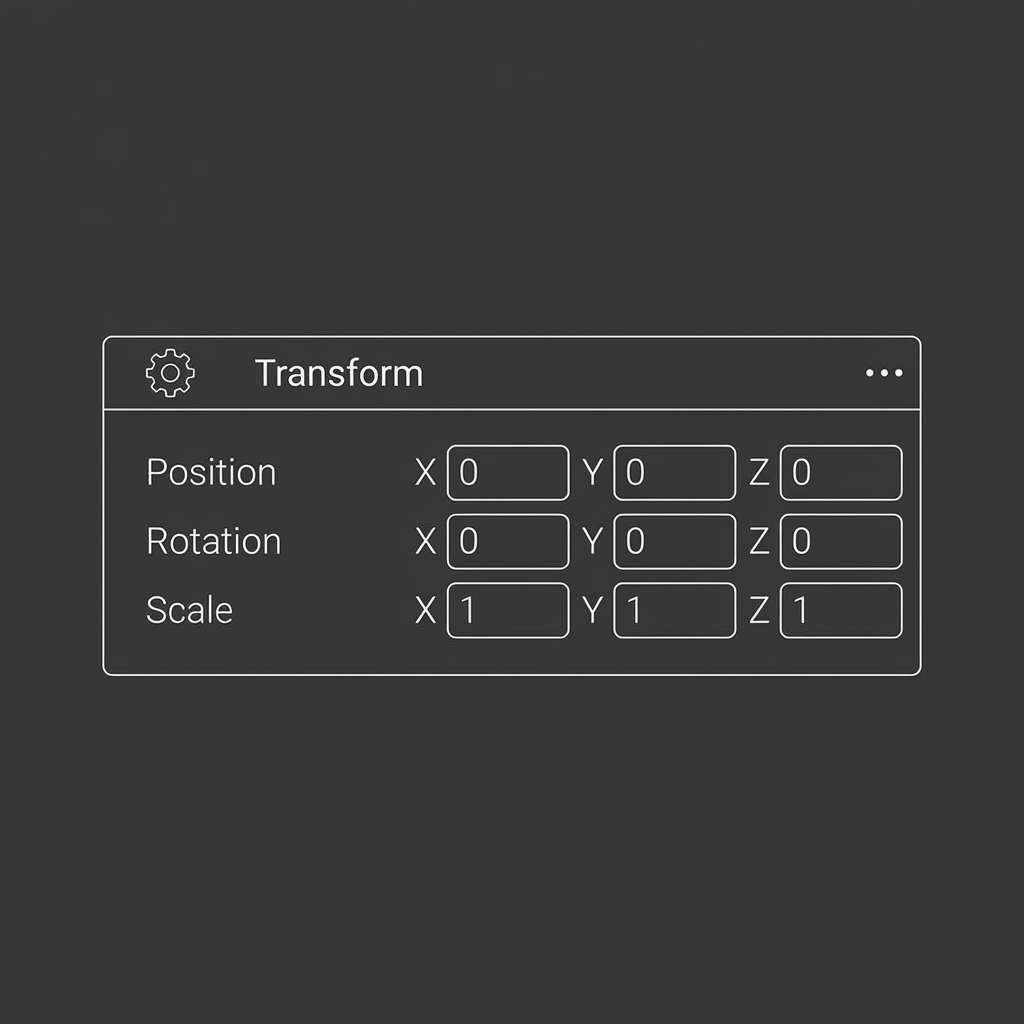
\includegraphics[width=0.6\textwidth]{figures/inspector_transform.png}
        \caption{Komponen Transform pada Inspector}
        \label{fig:inspector_transform}
    \end{figure}
    \item Ubah Scale menjadi $(0.5, 1, 1)$ agar bentuknya lebih menyerupai pesawat tempur ramping.
    \item Ubah warna melalui komponen \textbf{Sprite Renderer} (pilih warna hijau atau biru neon).
\end{enumerate}

\subsection{Mengatur Hierarki}

Agar pesawat terlihat lebih detail, kita bisa menambahkan \textit{Child Object} sebagai hiasan (misalnya knalpot mesin).

\begin{enumerate}
    \item Klik kanan pada objek \texttt{Player} > \textbf{Create Empty}. Beri nama \texttt{Engine}.
    \item Di dalam \texttt{Engine}, tambahkan Sprite \textbf{Square} kecil di bagian bawah pesawat.
    \item Perhatikan bahwa saat kita menggerakkan \texttt{Player}, objek \texttt{Engine} akan ikut bergerak. Ini adalah konsep \textbf{Parent-Child} dalam Unity.
\end{enumerate}

\begin{figure}[ht]
    \centering
    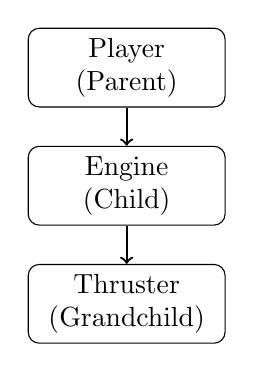
\begin{tikzpicture}[
        node distance=1.5cm,
        every node/.style={draw, rectangle, rounded corners, align=center, minimum width=2.5cm, minimum height=1cm}
    ]
        \node (player) {Player\\(Parent)};
        \node (engine) [below of=player] {Engine\\(Child)};
        \node (thruster) [below of=engine] {Thruster\\(Grandchild)};
        
        \draw[->, thick] (player) -- (engine);
        \draw[->, thick] (engine) -- (thruster);
    \end{tikzpicture}
    \caption{Ilustrasi Hierarki Parent-Child}
    \label{fig:parent_child}
\end{figure}

\begin{lstlisting}[language={[Sharp]C}, caption=Ilustrasi Hierarki Player]
- Player (Triangle)
  |- Engine (Empty)
     |- Thruster (Square)
\end{lstlisting}
